\documentclass{article}
\usepackage[utf8]{inputenc}
\usepackage{polski}
\usepackage{graphics}
\usepackage{graphicx}
\usepackage{mathtools}


\title{Sprawozdanie 1 Labolatorium Sterowania Procesami Ciągłymi }
\author{Jakub Michalski \\ 248973}
\date{23.10.2020 PT/TP $7^{15}$}

\begin{document}

\maketitle

\section{Wstęp}
Zadanie do wykonania polegało na przeanalizowaniu zachowania odpowiedzi skokowych z różnymi biegunami. Kolejnym zadaniem było zidentyfikowanie biegunów odpowiedzi skokowej na podstawie jej charakterystyki i charakterystyki jej pochodnej.

\section{Odpowiedzi skokowe dla różnego rozłożenia biegunów transmitancji}

Bieguny rzeczywiste ujemne. $s_1 = -2 , s_2 = -2$. Daje nam to układ stabilny bez oscylacji.

\begin{wrapfigure}
    \centering
    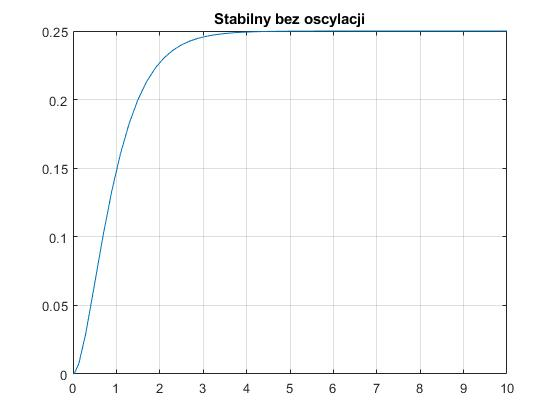
\includegraphics[width=0.5\textwidth]{stabbezosc.jpg}
\end{wrapfigure}
\begin{wrapfigure}
    \centering
    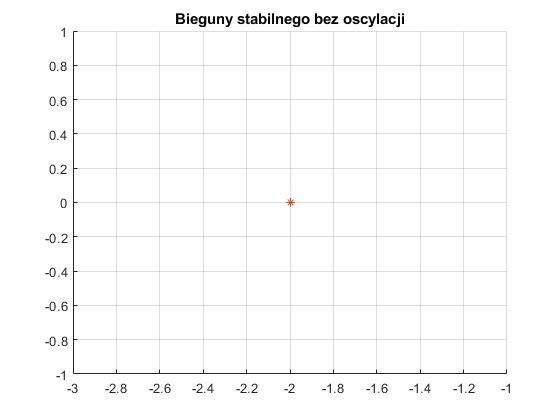
\includegraphics[width=0.5\textwidth]{biegstabbezosc.jpg}
\end{wrapfigure}
Wzrór transmitancji:

$$ K(s) =\frac{1}{s^2+4s+4} $$
\newpage

Bieguny rzeczywiste dodatnie. $s_1 = 2,s_2 = 2$. Daje nam to układ niestabilny bez oscylacji.

\begin{wrapfigure}
    \centering
    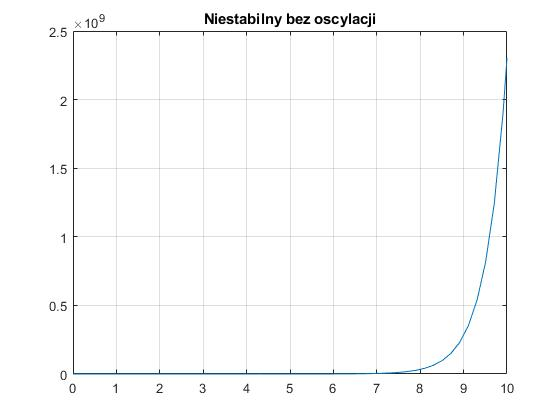
\includegraphics[width=0.5\textwidth]{niestab.jpg}
\end{wrapfigure}
\begin{wrapfigure}
    \centering
    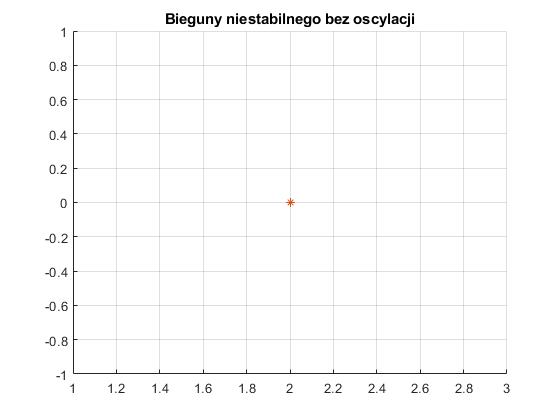
\includegraphics[width=0.5\textwidth]{biegniestab.jpg}
\end{wrapfigure}
Wzrór transmitancji:

$$ K(s) =\frac{1}{s^2-4s+4} $$

Bieguny urojone ujemne. $s_1 = -\frac{1}{2}+4j , -\frac{1}{2}-4j$. Daje nam to układ stabilny z oscylacji.

\begin{wrapfigure}
    \centering
    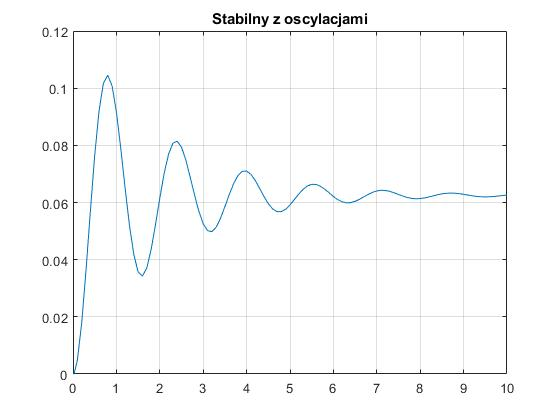
\includegraphics[width=0.5\textwidth]{stabosc.jpg}
\end{wrapfigure}
\begin{wrapfigure}
    \centering
    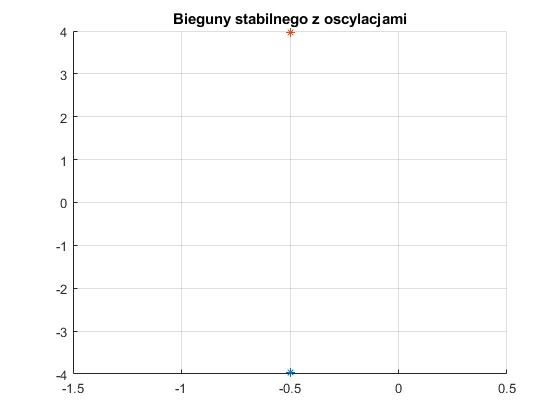
\includegraphics[width=0.5\textwidth]{biegoscstab.jpg}
\end{wrapfigure}
Wzrór transmitancji:

$$ K(s) =\frac{1}{s^2+s+16} $$
\newpage
Bieguny urojone dodatnie. $s_1 = \frac{1}{2}+4j , \frac{1}{2}-4j$. Daje nam to układ niestabilny z oscylacji.

\begin{wrapfigure}
    \centering
    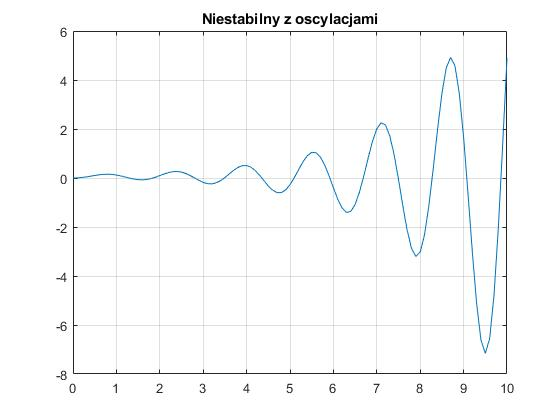
\includegraphics[width=0.5\textwidth]{oscniestab.jpg}
\end{wrapfigure}
\begin{wrapfigure}
    \centering
    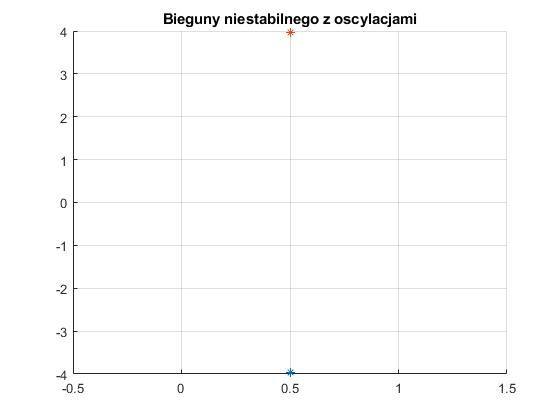
\includegraphics[width=0.5\textwidth]{biegoscniestab.jpg}
\end{wrapfigure}
$$ K(s) =\frac{1}{s^2-s+16} $$

\section{Identyfikacja}
Badaną funkcją jest $ K(s) =\frac{1}{s^2-s+10} $. Biorąc dane z charakterystyki odpowiedzi skokowej i z jej pochodnej mozemy wyznaczyć okres oraz potrzebne punkty. $T = 2.65 - 0.6 = 2.05, A = [0.5,0.2511] B = [2.5,0.0917]$.
Wartość $B_t$ zmieniona w porównaniu do tej na wykresie by wartosci były na tej samej linni. Wynika to z niedokładnosci w próbkowaniu.

\begin{wrapfigure}
    \centering
    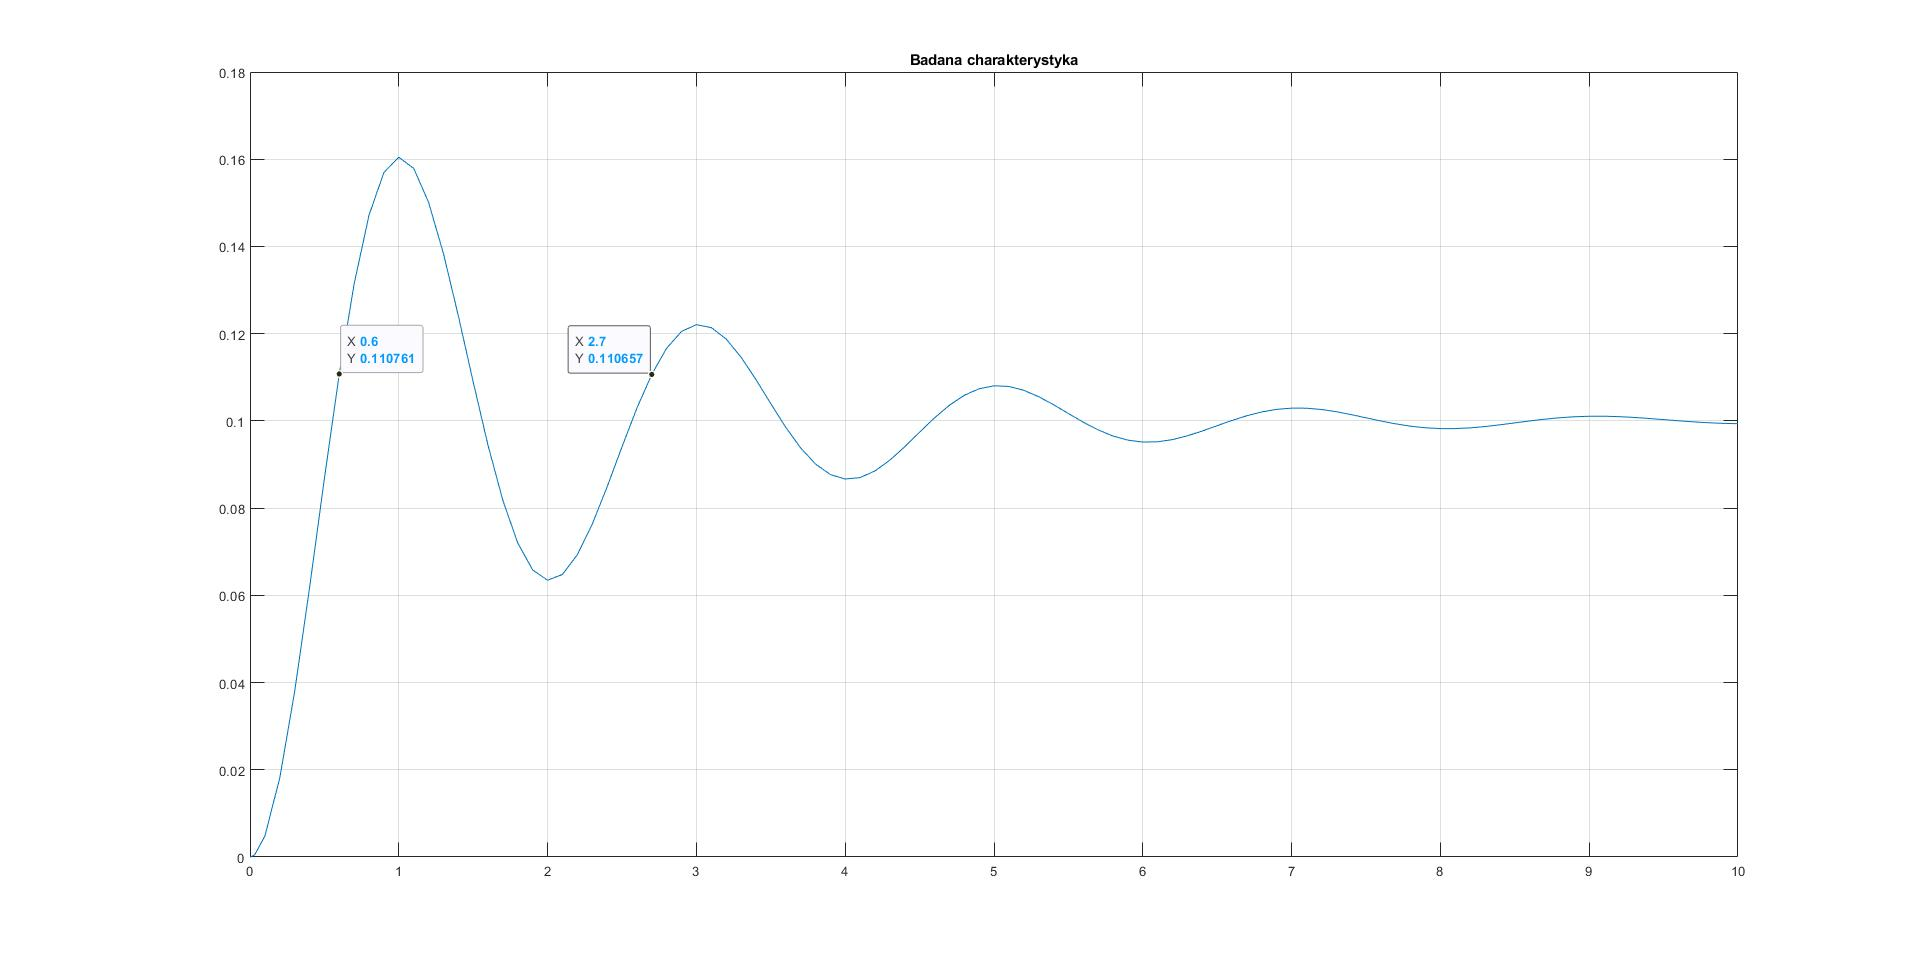
\includegraphics[width=13cm]{odp.jpg}
\end{wrapfigure}

\begin{wrapfigure}
    \centering
    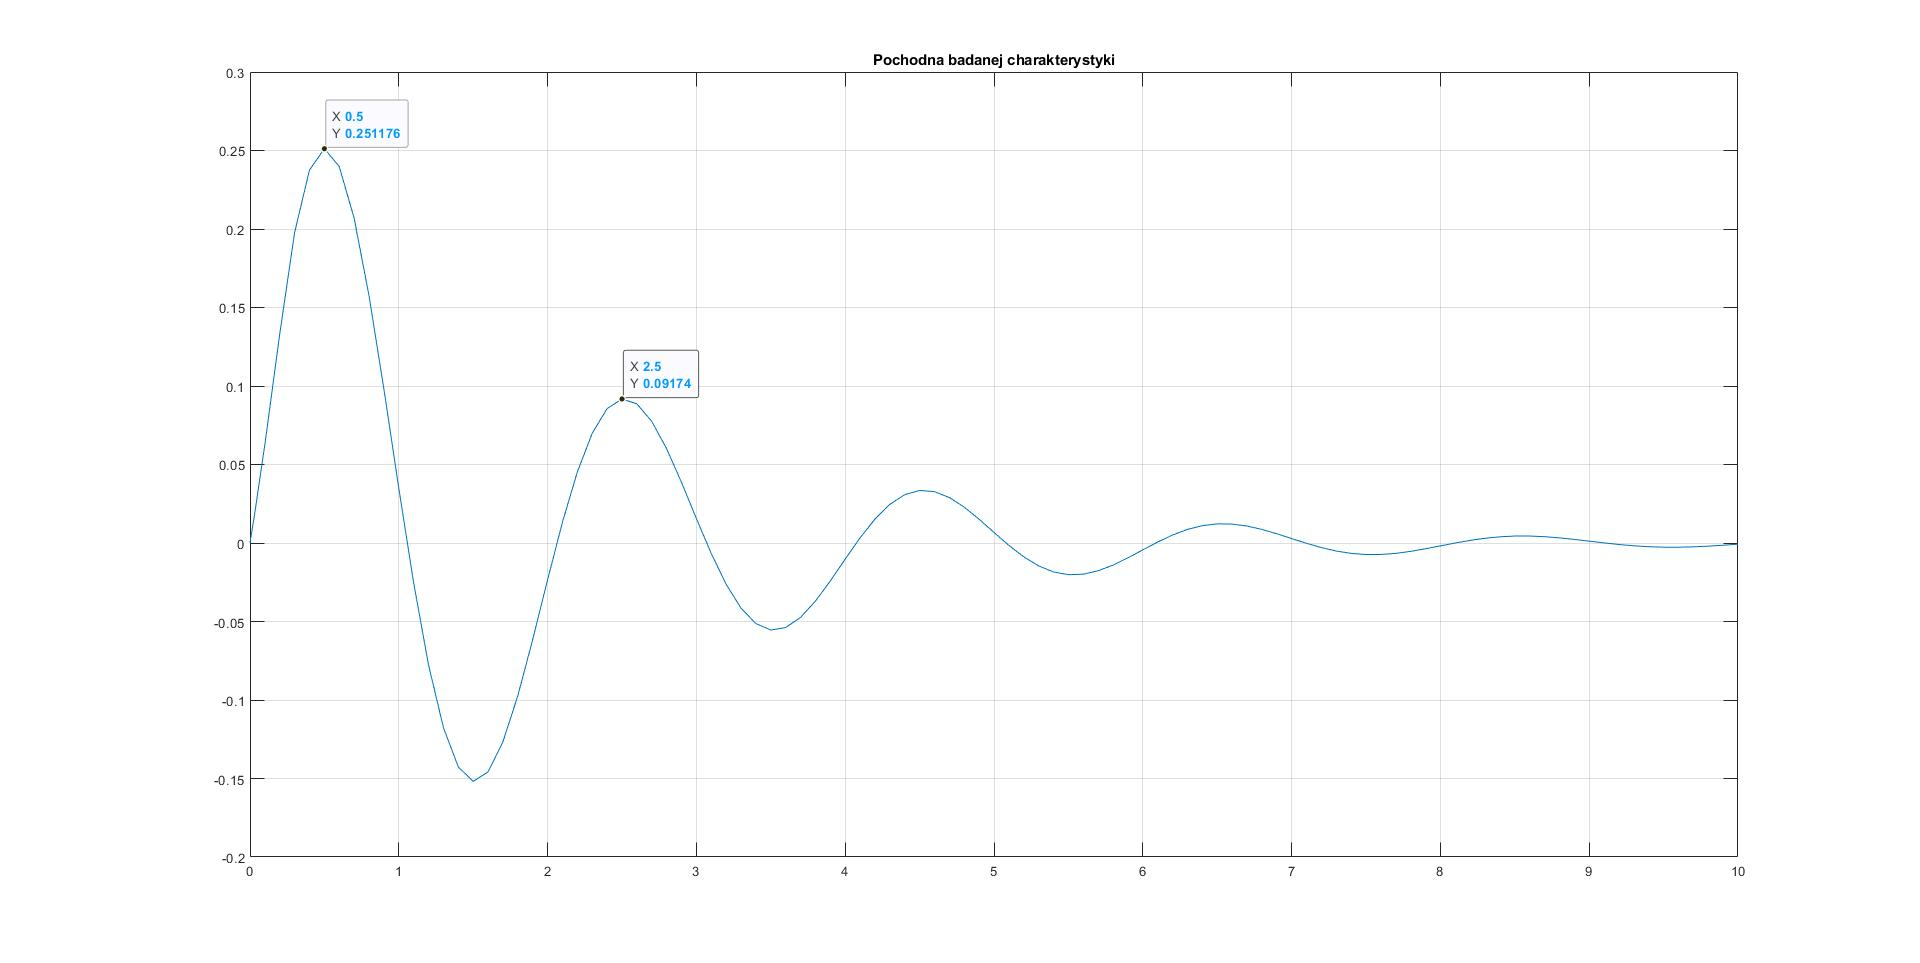
\includegraphics[width=13cm]{odpimp.jpg}
\end{wrapfigure}

Na podstawie wzoru ogólnego odpowiedzi skokowej, jesteśmy w stanie wyznaczyć bieguny badanego obiektu.
$$
    \lambda(t) = 2|\alpha|e^\sigma^t cos(\omega t + \phi)  
$$
Jako ze A i B są maksymami lokalnymi to $cos(\omega t + \phi) = 1$

\centering
\bigg\{
\begin{tabular}{cc}
          & $ A_y = 2|\alpha|e^\sigma^{A_t} $ \\
          & $B_y = 2|\alpha|e^\sigma^{B_t}$
\end{tabular}

\raggedright

Na podstawie wzoru możemy obliczyć część rzeczywistą obiektu:
$$
\sigma = \frac{ln(\frac{B_y}{A_y})}{B_t-A_t}=\frac{ln(\frac{0.0917}{0.2511})}{2.5-0.5} = -0.5037
$$

Znając okres odpowiedzi  możemy obliczyć część urojoną obiektu:

$$
\omega = \frac{2\pi}{T} = \frac{2\pi}{2.65-0.6} = 3.0634
$$

Na podstawie tej analizy mozemy powiedzieć ze s1 i s2 wyglądają następująco:
$$
    s_{12}= -0.5037\pm 3.0634j
$$

Po podstawieniu do wzoru wykonane obliczenia otrzymujemy dany wzór:

$$
 K(s) =\frac{1}{s^2-s+9.6382} \approx  \frac{1}{s^2-s+10}
$$
\newpage
\section{Wnioski}
\subsection{}
Zachowanie charakterystyki zależy od położenia biegunów. Jeżeli wartość rzeczywista bieguna jest dodatnia świadczy to o niestabilnosci. Dopiero gdy wartość rzeczywista wszystkich biegunów jest ujemna to układ jest stabilny. Część urojona biegunów wprowadza oscylacje do układu.
\subsection{}
Posiadając charakterystyke odpowiedzi skokowej z oscylacjami ,oraz pochodną odpowiedzi skokowej jesteśmy w stanie w przyblizeniu wyliczyć bieguny układu oraz jego transmitancje.


\end{document}
